\documentclass[10pt,a4paper,final]{article}
%
\usepackage[utf8x]{inputenc}
\usepackage{ucs}
\usepackage{amsmath}
\usepackage{geometry}
\usepackage{anysize} % Soporte para el comando \marginsize
\usepackage{graphicx}
\usepackage{amsfonts}
\usepackage{amssymb}
\usepackage[spanish]{babel}
%%%%%%%%%%%%%%%%%%%%%%%%%%%%%%%%%%%%%%%%%%%%%%%%%
%%%%%%%%%%%%%%%%%%%%%%%%%%%%%%%%%%%%%%%%%%%%%%%%%
%%%%%%%%%%%%%%%%%%%%%%%%%%%%%%%%%%%%%%%%%%%%%%%%%
\marginsize{2cm}{2cm}{1.5cm}{1.5cm}
%
\begin{document}
\title{Calculo de descensos en un campo de bombeo en medios porosos}
\author{Christian N. Pfarher, Juan Pablo Garbarino, Marina Castro\\
\textit{Trabajo práctico final de ``Métodos numéricos y simulación'', II-FICH-UNL.}}
\markboth{Método numérico y simulación: TRABAJO FINAL}{}
\date{\today}
\maketitle
%%%%%%%%%%%%%%%%%%%%%%%%%%%%%%%%%%%%%%%%%%%%%%%%%
%%%%%%%%%%%%%%%%%%%%%%%%%%%%%%%%%%%%%%%%%%%%%%%%%
%%%%%%%%%%%%%%%%%%%%%%%%%%%%%%%%%%%%%%%%%%%%%%%%%
\newpage
\tableofcontents
%%%%%%%%%%%%%%%%%%%%%%%%%%%%%%%%%%%%%%%%%%%%%%%%%
%%%%%%%%%%%%%%%%%%%%%%%%%%%%%%%%%%%%%%%%%%%%%%%%%
%%%%%%%%%%%%%%%%%%%%%%%%%%%%%%%%%%%%%%%%%%%%%%%%%
\newpage
%%%%%%%%%%%%%%%%%%%%%%%%%%%%%%%%%%%%%%%%%%%%%%%%%
%%%%%%%%%%%%%%%%%%%%%%%%%%%%%%%%%%%%%%%%%%%%%%%%%
%%%%%%%%%%%%%%%%%%%%%%%%%%%%%%%%%%%%%%%%%%%%%%%%%
\section{Introducción}
En el presente trabajo, se presentan los resultados de la simulación de un campo de bombeo en medios porosos. El campo
consta de 2 pozos de bombeo de agua que funcionan por 15 horas seguidas. 

Para la realización del trabajo se utilizó el software de pre y pos proceso GiD \footnote{http://gid.cimne.upc.es/}. Mediante el mismo, se utilizó el \emph{módulo de pre-proceso} para la carga de los datos del problema, mientras que para
la simulación se utilizó Tdyn \footnote{es un entorno tridimensional de análisis fluidodinámico (CFD) y multifísica basado en el método de los elementos finitos estabilizado}(\emph{módulo de post-proceso}).
%%%%%%%%%%%%%%%%%%%%%%%%%%%%%%%%%%%%%%%%%%%%%%%%%
%%%%%%%%%%%%%%%%%%%%%%%%%%%%%%%%%%%%%%%%%%%%%%%%%
%%%%%%%%%%%%%%%%%%%%%%%%%%%%%%%%%%%%%%%%%%%%%%%%%
\section{Objetivos}
El objetivo de este trabajo, consiste en la simulación de lineas de corrientes y equipotenciales en un campo de bombeo (medio poroso) con 2 bombas de extracción de agua en un acuífero libre (no confinado), homogéneo e isótropo.

%%%%%%%%%%%%%%%%%%%%%%%%%%%%%%%%%%%%%%%%%%%%%%%%%
%%%%%%%%%%%%%%%%%%%%%%%%%%%%%%%%%%%%%%%%%%%%%%%%%
%%%%%%%%%%%%%%%%%%%%%%%%%%%%%%%%%%%%%%%%%%%%%%%%%
\section{Base Teórica}
básicamente es la ecuación de poisson con k
representado la permeabilidad.
%
\subsection{Modelo matemático o fisico.. ver}
describir mod mate.
 son las ecuaciones matemáticas, en nuestro caso las
ecuaciones de navier stokes
%
\subsection{Modelo numérico}
describir mod num.
tdyn resuelve en el espacio por el método de
elementos finitos y 
temporalmente hay que fijarse que opción está
tildada. *************************************************ver*******************************************
%%%%%%%%%%%%%%%%%%%%%%%%%%%%%%%%%%%%%%%%%%%%%%%%%
%%%%%%%%%%%%%%%%%%%%%%%%%%%%%%%%%%%%%%%%%%%%%%%%%
%%%%%%%%%%%%%%%%%%%%%%%%%%%%%%%%%%%%%%%%%%%%%%%%%
\section{Desarrollo}
\subsection{Datos del problema}
Los datos que se pudieron obtener del problema son:
\begin{itemize}
	\item Discretización del área a modelar:	
	\begin{itemize}
		\item Dominio: $x=1000 ~m.$, $y=1000 ~m.$
		\item Acuífero libre, homogéneo e isótropo $(K_x = K_y = K_z)$
		\item Espesor del acuífero: $20 ~m.$*
	\end{itemize}
	%
	\item Ubicación de los Pozos de bombeo:
	\begin{itemize}
		\item Pozo Bombeo 1: $x=150~m.$, $y=650 ~m.$
		\item Pozo Bombeo 2: $x=750~m.$, $y=250 ~m.$
	\end{itemize}
	%
	\item Caudal de bombeo:
	\begin{itemize}
		\item Pozo Bombeo 1: $60~m³/h$
		\item Pozo Bombeo 2: $40~m³/h$
		%\item[] Ambos posos trabajan 15 horas por día
	\end{itemize}
	\item Filtro: Tramo filtrante de $15~m.$ de longitud*
	\item Transmisividad: $600~m²/d$
	\item Coeficiente de almacenamiento: $5*10⁻²$ \begin{LARGE}
	creo que este no lo usamos... ver
	\end{LARGE}
	\item Porosidad efectiva: $5*10⁻²$
\end{itemize}
* Debido a problemas que se explican en el desarrollo del presente trabajo hay que aclarar que tanto el tramo filtrante como el espesor del acuífero se aumentó en un factor de 10, es decir los valores finales fueron de $150 m.$ y $200 m.$ respectivamente.
%
\subsection{Definición de Geometría}
Para la geometría en tres dimensiones se tiene los siguientes datos:
En las figuras \ref{cotas_superiores_generalesXY}, \ref{cotas_superiores_detallesXY} y \ref{cotas_grales_YZ} se pueden observar
las dimensiones de las geometrías según los datos del problema. Hay que aclarar aquí que el cuadrado de $300~m.~x~300~m.$ que se visualiza
en la figura \ref{cotas_superiores_detallesXY} como el rectángulo de $400~m.~x~300~m.$ en la misma figura, solo fueron dibujados con el
objetivo, de a posteriori, realizar un refinamiento del dominio en la zona que más intereza visualizar.\\
\begin{itemize}
\item Número de puntos: 33
\item Número de lineas: 52
\item Número de superficies: 28
\item Número de volumenes: 3
\end{itemize}
***************************
aclarara aca lo de los redimensioneamientos y demas...
***************************
\begin{figure}[tbhp]
\centerline{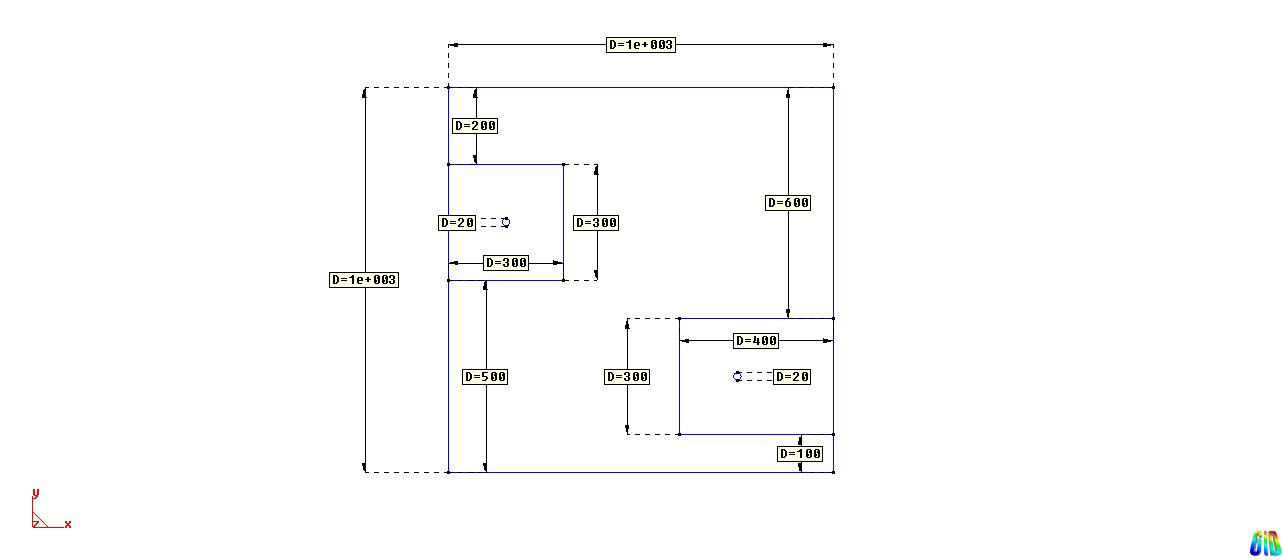
\includegraphics[scale=0.75]{img/cotas_superiores_generalesXY}}
\caption{Vista General de las cotas en el Plano XY}
\label{cotas_superiores_generalesXY}
\end{figure}

%
\begin{figure}[tbhp]
\centerline{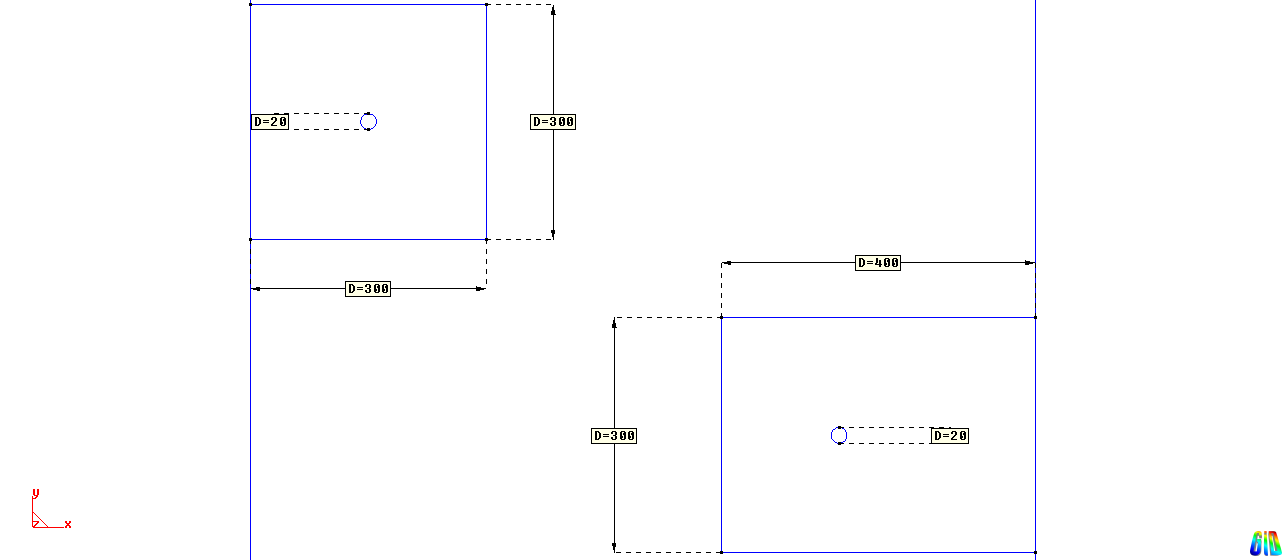
\includegraphics[scale=0.75]{img/cotas_superiores_detallesXY}}
\caption{Vista en detalle (pozos) de las cotas en el Plano XY}
\label{cotas_superiores_detallesXY}
\end{figure}
%

%
\begin{figure}[tbhp]
\centerline{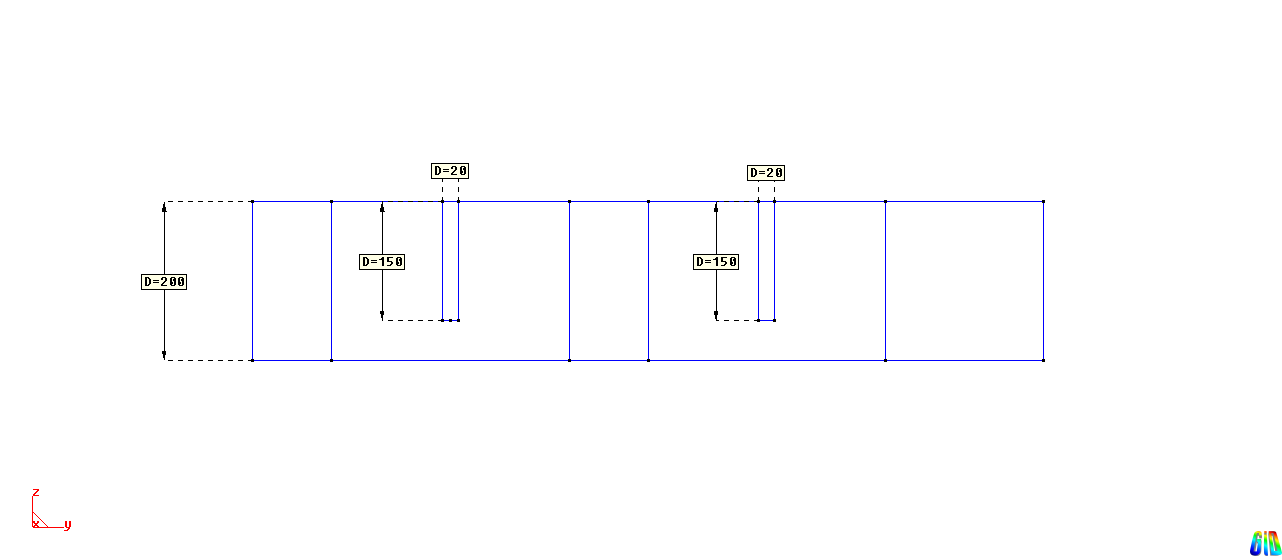
\includegraphics[scale=0.75]{img/cotas_grales_YZ}}
\caption{Vista en de las cotas en el plano YZ}
\label{cotas_grales_YZ}
\end{figure}
%
En la figura \ref{superficies_y_volumenes} se pueden observar las generaciones de las superficies (color magenta) y volúmenes (color cyan)
de la geometría.
%
\begin{figure}[tbhp]
\centerline{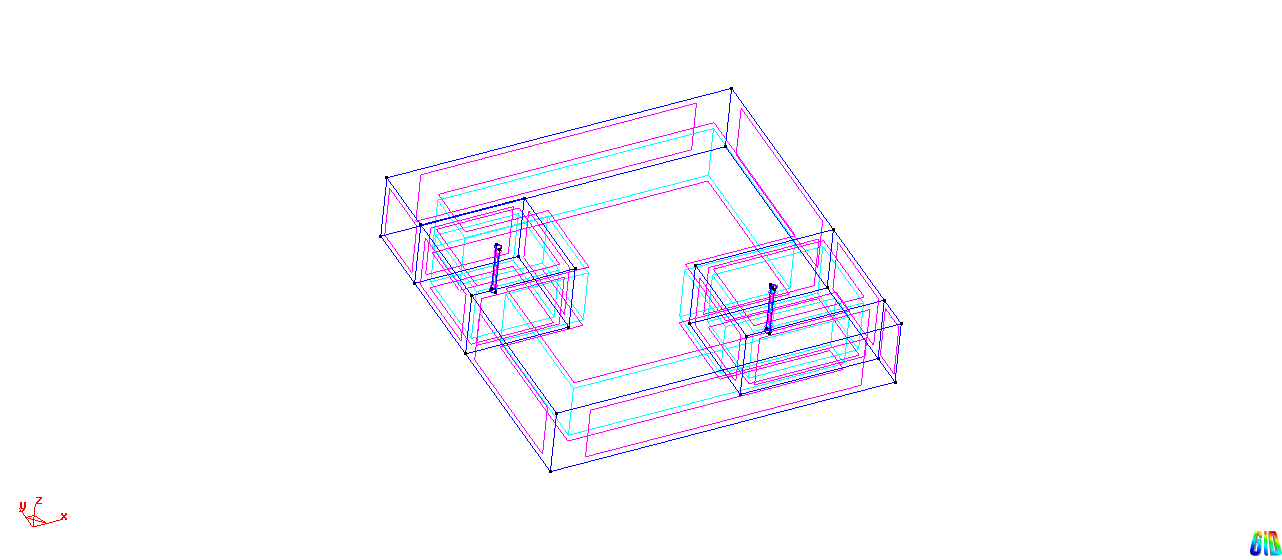
\includegraphics[scale=0.75]{img/superficies_y_volumenes}}
\caption{Superficies y Volúmenes de la Geometría}
\label{superficies_y_volumenes}
\end{figure}
%
%
%%
%\begin{figure}[tbhp]
%\centerline{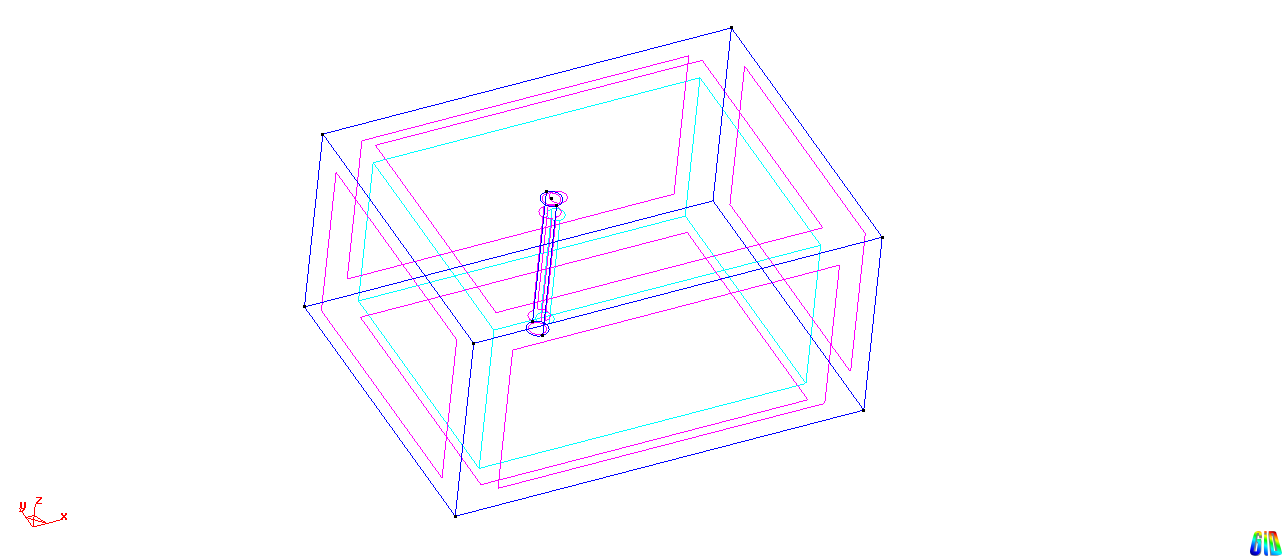
\includegraphics[scale=0.75]{img/detalle_pozo2_sup_vol}}
%\caption{Vista en detalle de las superficies y volúmenes generados (pozo 2)}
%\label{detalle_pozo2_sup_vol}
%\end{figure}
%%
%
%%
%\begin{figure}[tbhp]
%\centerline{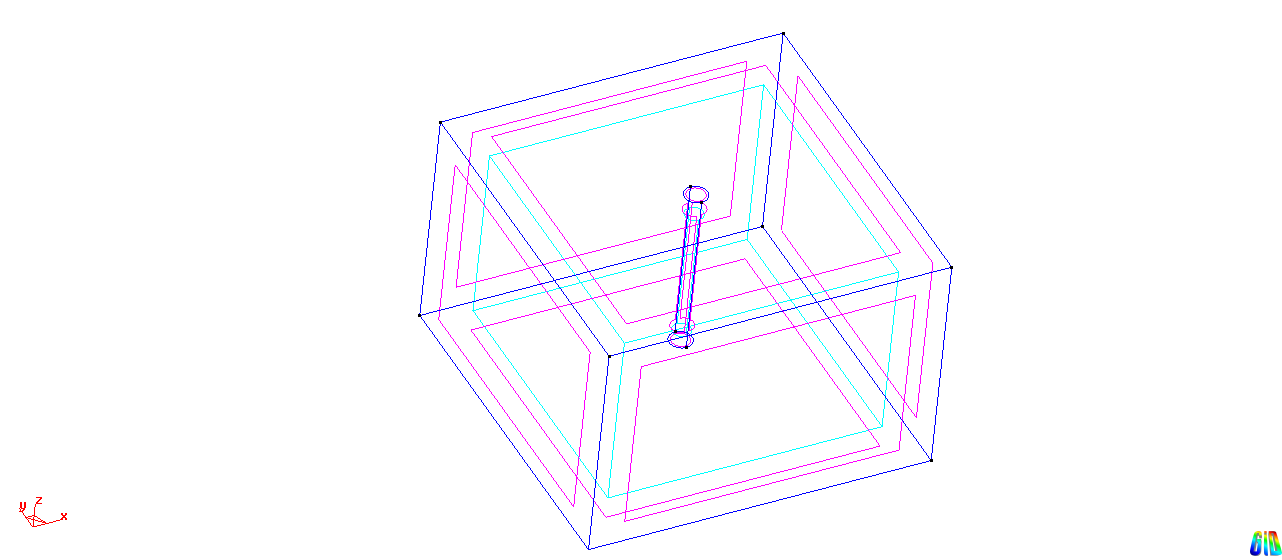
\includegraphics[scale=0.75]{img/detalle_pozo1_sup_vol}}
%\caption{Vista en detalle de las superficies y volúmenes generados (pozo 1)}
%\label{detalle_pozo1_sup_vol}
%\end{figure}
%%

%
\subsection{Propiedades del medio y de los materiales}
A partir de los datos del problema se tuvieron que realizar conversiones de unidades y el cálculo de diferentes valores para ser ingresados en el programa GID.
%
\subsubsection{Material Suelo}
En la pestaña ransol de la ventana de materiales de fluidos para el material suelo de  se introdujeron los siguientes valores:
\begin{itemize}
\item Modelo de Fluido: Incompressible
\item Densidad: $999.7~Kg/m^3$ (agua a $10° C$) \footnote{ según datos obtenidos de Tabla-libro ...}
\item Viscosidad: $0.001307~Pa.s$ (agua a $10° C$)\footnote{ según datos obtenidos de Tabla-libro ...}
\item Resistencia de la Ley de Darcy:
quizas explicar que corno y como se haya este coeficiente de 0.0000017 y que representa la ley de darcy.. porosidad del suelo...\\
silvina: Ley de resistencia de darcy: es la ley que habla de la velocidad que tiene el agua para moverse dentro del medio poroso. Hay 6 valores porque este coef puede ser homogeneo en todo el suelo, esto se llama suelo isotropico, es el que tiene el mismo coef de trasmisividad en todos los sentidos: x,y,z. Cuando el suelo tiene distinto coef se usa toda la matriz que es lo real y lo normal. A los fines del cálculo lo usamos como isotropico, entonces solo completamos la diag principal y con el mismo valor (hay que ver el tema de la unidad, porque esta distinta a los datos). 
\begin{equation}
\begin{pmatrix}{}
0.0000017 & 0.0 & 0.0 \\ 
0.0 & 0.0000017 & 0.0 \\ 
0.0 & 0.0 & 0.0000017
\end{pmatrix} 1/m²
\label{matrizdarcys}
\end{equation}
Debido a que se está en presencia de un acuífero isótropo, en (\ref{matrizdarcys}) se puede observar que sólo la diagonal principal de la matriz tiene valores diferentes de cero.
\end{itemize}
En la figura \ref{datos_materiales_suelo_vista} se puede observar la asignación del material definido a la parte del dominio correspondiente.

\begin{figure}[tbhp]
\centerline{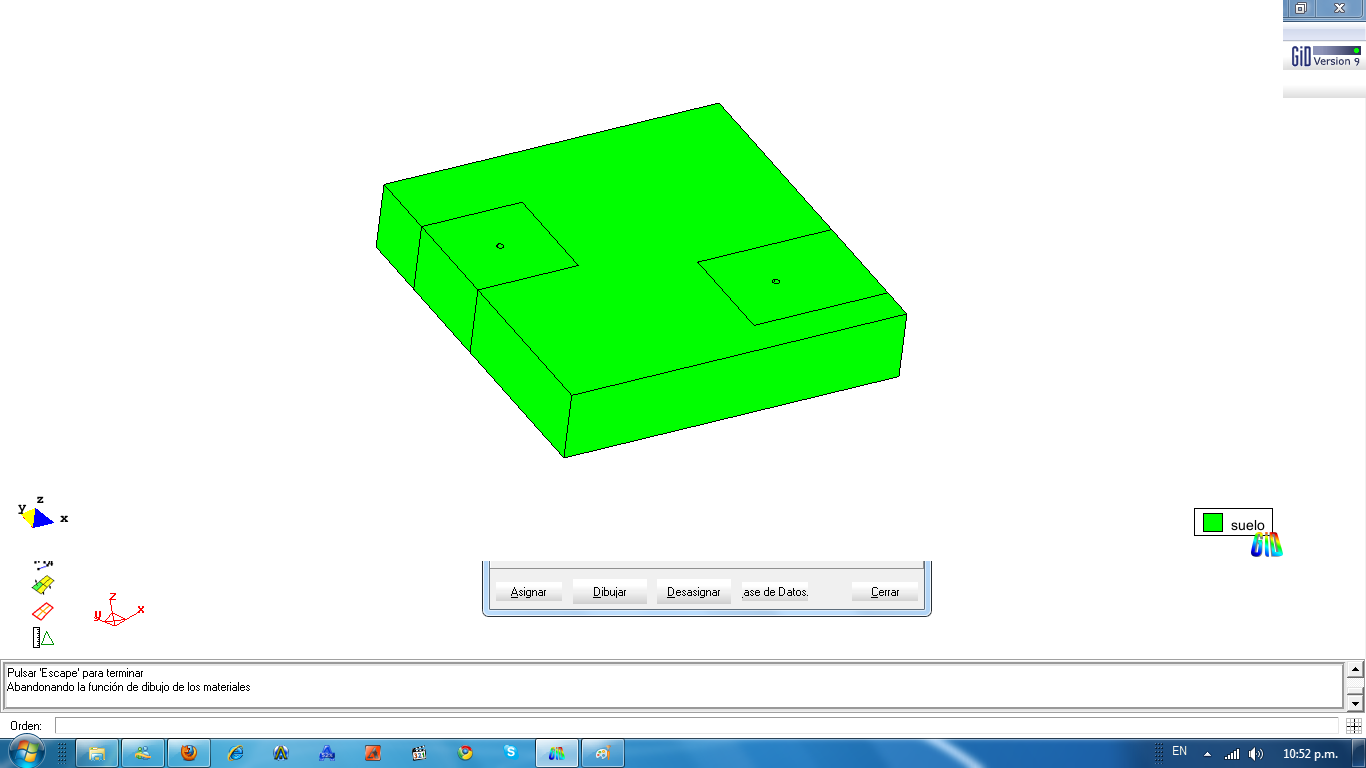
\includegraphics[scale=0.75]{img/datos_materiales_suelo_vista}}
\caption{Material Suelo asignado a la geometría}
\label{datos_materiales_suelo_vista}
\end{figure}

Características de Fluido: Flujo laminar, se comporta como viscoso por la velocidad lenta. \begin{LARGE}
que onda esto????
\end{LARGE} 
%
\subsubsection{Material Wall o Pared}
En la ventana de contornos fluidos se asigno a las paredes de ambos pozos el contorno definido por defecto Wall. El tipo de contorno seleccionado fue el \emph{V fixWall} con el ángulo por defecto de $60°$. Este es el modelo elegido en Tdyn para simular el comportamiento del flujo en las paredes del dominio. Básicamente, impone que la velocidad en las superficies asignadas será nula, "simulando" así la pared del pozo por la que no existe penegración de agua. En la figura \ref{datos_contornos_fluidos_vista} se puede observar el material asignado a ambos pozos.
\begin{figure}[tbhp]
\centerline{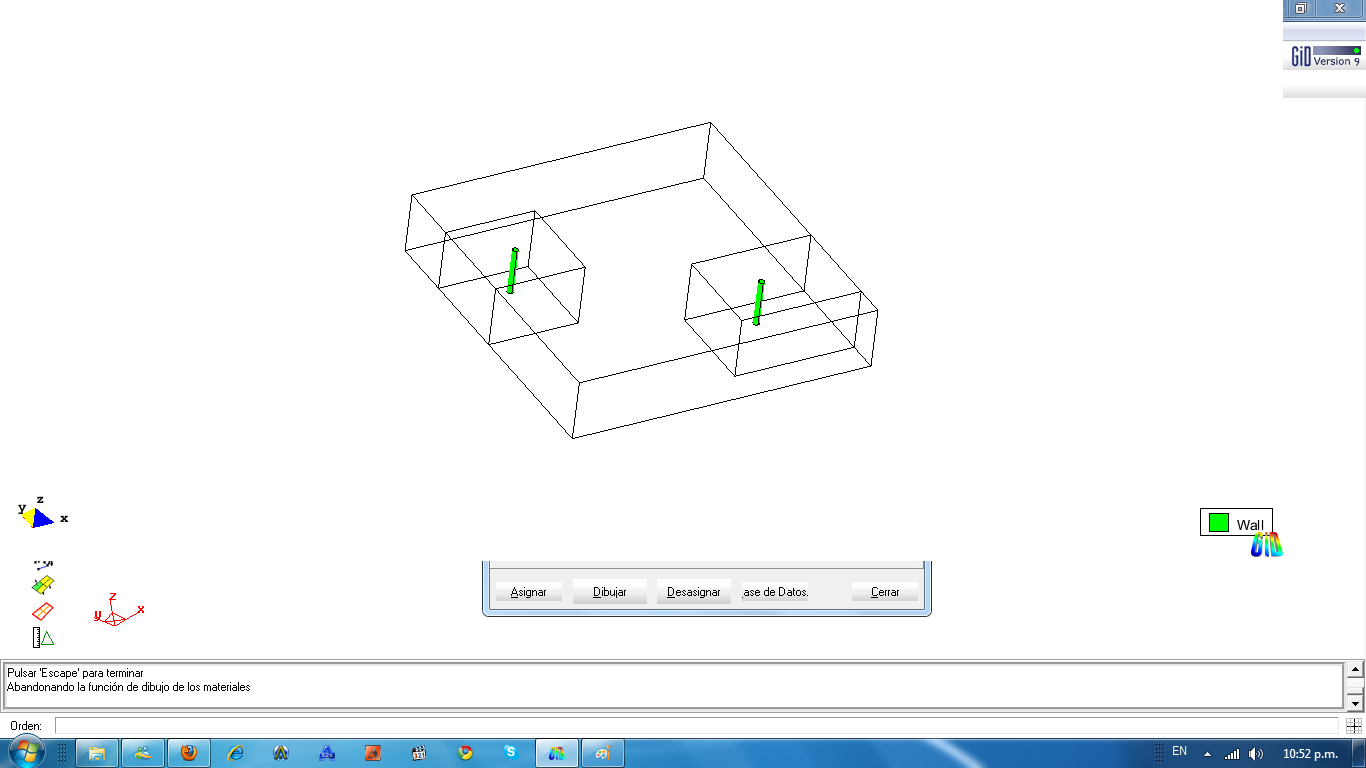
\includegraphics[scale=0.75]{img/datos_contornos_fluidos_vista}}
\caption{Material Wall o Pared asignado a la geometría}
\label{datos_contornos_fluidos_vista}
\end{figure}

%
\subsection{Condiciones de borde}
Para fijar las condiciones de borde, se procedió mediante el menú datos -> condiciones -> ransol. Luego se selecciono la opción de asignación de propiedades a superficies y se procedió a fijar las diferentes condiciones:
\begin{figure}[tbhp]
\centerline{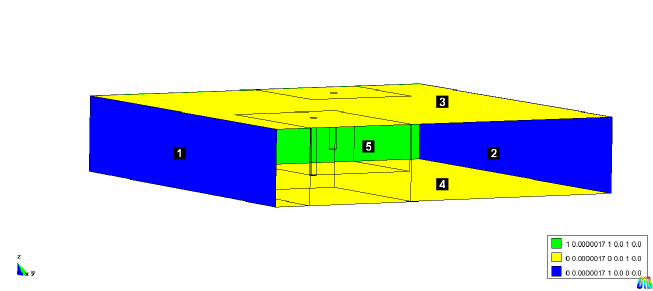
\includegraphics[scale=0.75]{img/datos_condiciones_ransol_fijar_velocidadinterno_leyendas}}
\caption{Velocidades Fijas}
\label{datos_condiciones_ransol_fijar_velocidadinterno_leyendas}
\end{figure}
\subsubsection*{Fijar Velocidad}
Como se puede ver en la figura \ref{datos_condiciones_ransol_fijar_velocidadinterno_leyendas} las condiciones asignadas a cada una de las superficies enumeradas son las siguientes:
\begin{enumerate}
\item Superficie 1 y 2:
\begin{eqnarray*}
Fija~V_x&=&0.0000017~[m/s]\\
Fija~V_y&=&0.0~[m/s]\\
Fija~V_z&=&0.0~[m/s]\\
\end{eqnarray*}
\item Superficie 3 y 4:\begin{eqnarray*}
V_x&=&0.0000017~[m/s]\\
V_y&=&0.0~[m/s]\\
Fija~V_z&=&0.0~[m/s]
\end{eqnarray*}
\item Superficie 5:
\begin{eqnarray*}
V_x&=&0.0000017~[m/s]\\
Fija~V_y&=&0.0~[m/s]\\
V_z&=&0.0~[m/s]
\end{eqnarray*}
\end{enumerate}
\subsubsection*{Fijar Presión}
En la figura \ref{datos_condiciones_ransol_presion} se puede observar que se fijó un valor de referencia para la presión en la superficie del extremo final de salida del campo con valor igual a $0.0~Pa$. Esto significa que los resultados que obtendremos para la presión serán relativos a esta condición.

\begin{figure}[tbhp]
\centerline{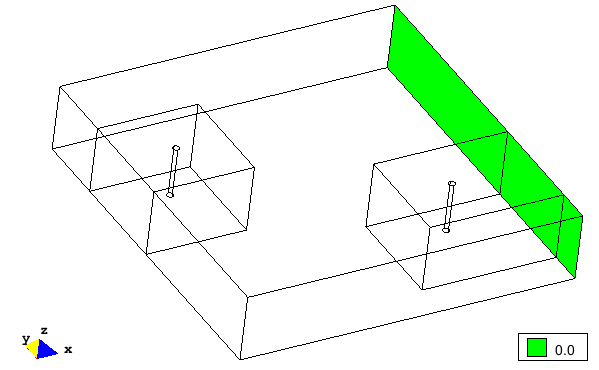
\includegraphics[scale=0.75]{img/datos_condiciones_ransol_presion}}
\caption{Condición fija de presión}
\label{datos_condiciones_ransol_presion}
\end{figure}

\subsubsection*{Campo de Velocidad}

(velocidad de campo) Libre x,libre y. Porque incorporo componentes los valores estan incoroprados en data.
que deslice en x y y..(fijamos z).
el flujo puede ir volver avanzar y retroceder pero no puede subir y bajar. El value field esta en 0 porque lo calcula el codigo.. al no fijarlo el codigo lo calcula
el moviemiento va a ser adentro del dominio. se lo asigno  a la superficie de arriba
**************************************************************************************************
En los softwares específicos de hidrogeología, fijate que aca tenes el esquema de calculo que es una malla muy guresa en dos dimensiones, que te va a dar isocurvas de niveles. Se va a ver como esto va bombeando y ese nivel de agua cerca de la bomba va ir deprimiendose formando el cono de desenso. Eso, asi de esa forma aca no lo vamos a poder hacer, porque para poder hacer eso en 3D (en 2D si se puede) tenes que tener un soft que distinga entre suelo no saturado y suelo saturado. En el suelo saturado las ecs de gobierno son distintas a las del no saturado. El soft que tenemos solamente tiene las ecs de gob del suelo saturado, el no saturado tiene un modelo mucho mas complejo, en realidad estos modelos son bidimensionales porque no calculan el flujo en suelo saturado, lo que calculan seria la curva, la interfaz, seria la sup que los separa, nada mas, sería la ubicación de esa sup que distingue zona saturada de la no saturada. que tiene ecuaciones simples, pero no calcula detalles del flujo, este modelo calcula el flujo en suelo saturado. 

Se coincidiera que se esta en presencia de un estrato de suleo saturado (esto es saturado de agua). 
Vamos a tener lineas equipotenciales (unen lineas de igual potencial hidráulico) las cuales son perpendiculares a las lineas del flujo y serian valores de presión que ejerce el agua sobre el suelo. Esas líneas equipotenciales van a ser equivalentes en interpretacion a las lineas de superficie que se calculan tradicionalmente en hidrologia.

Coef de trasmisividad: cuanto mas chiquito es mas lento se mueve el agua en el suelo.

Tenes las propiedades del suelo, que serian equivalentes a los parametros del modelo, los parametros de las ecuaciones de gobierno; Y las condiciones de borde serían los valores de contorno, de arranque (son particulares del problema).

El fluído es incompresible. La densidad y viscosidad del agua se saca en función de la temperatura, que le pongan a 10 grados la viscosidad está bien... 1 y 1 como está por defecto no, es muy viscoso eso... Esto serían las propiedades del material que son los parámetros del modelo, ahora falta poner los caudales de salida, problem data-->conditions-->ransol.., acá vamos a aplicar este caudal de bombeo, acá ya sabemos que este caudal es variante en el tiempo, pero acá no podemos poner esos datos, las condiciones en este modelo se ingresan como velocidad o como presión, entonces podemos poner una presión negativa para arriba que chupe, o una velocidad de salidad, hay que ver, yo se que para estos casos gerardo estuvo haciendo calculos y por ahi alguno es medio conlfictivo, podemos empezar probando con velocidad. La velocidad la sacamos con Caudal= velocidad por area. El area es la del pozo. <Acá esta la duda de que diámetro tenían los pozos... creo terminamos poniendo 0,5>. 

[20:55]
Adentro del tubo no hay suelo, hay agua, el tubo va a tener un material distinto. Todo el suelo va a tener un valor del coef <trasmisividad?> determinado que lo tenemos que sacar... pero ahi adentro no va a haber suelo, entonces todos estos parámetros van a ser cero. Cuando asigamos esos parametros al suelo se le asigna al volumen, no a la sup. Ahí ya establece los valores de viscocidad a 0 grados..., 25, pero esto aca no lo pongan asi como esta, copienlo porque no andaba muy bien, copien para 25 grados la densidad, la viscocidad en 8,6. A esto copienlo y crean una capa que se llama fluido y ahi ponen esos valores. <Aca le preguntamos si a 25 grados, porque antes habia dicho 10 y dijo que si, porque es mas o menos lo mismo, no varia tanto, en realidad sería la temp que esta el agua>. Esta sería la capa fluido, esto se le asigna al volumen del pozo.

<Aca habia un problema con el volumen del pozo>

vamos a material-->fluid y ahi lo asignas con las propiedades del agua, en este caso la matriz te queda en cero porque es agua, lo unico que variaria es la viscocidad segun la temp. Despues crean uno nuevo "suelo" y lo hacemos para el campo y ponen los valores, hay que ver que valor trasmisividad le ponemos, esto va al volumen de todo el campo, los cubos de los pozos tambien.

Al valor de velocidad se lo ponemos en la superficie de arriba. Entonces a esta superficie le van a poner un valor de velocidad que va para arriba.

[39:00]
Esto hay que aplicarlo con condition--> ransol porque usamos fluido. Entonces donde ponen las condiciones para ransol le muestra todas opciones. Como condicion podemos poner la vel o la presion, la vel se puede reemplazar en este caso por una presion negativa (hay valores equivalentes). Elegimos superficie para fijar la velocidad, no fijamos la velocidad en el volumen porque dejamos que el programa lo calcule. En una simulacion, el lugar donde vos queres observar que pasa, ese lugar no tiene que tener condiciones, las cond tienen que estaar lo suficientemente alejadas para que esa condicion que es fija y que termina siendo no tan real, que esa parte no tan real de tus condiciones no influya en lo que vos queres ver... Aca seleccionas superficie, fijar velocidad y fijamos en las 3 dimensiones, en z sería el valor ese. Seria positivo porque es hacia arriba.

La pared del cilindro va a ser una barrera fisica porque afuera del cilindro esta el suelo, y el agua quieta cuando la bomba empiece a funcionar va entrar a moverse hacia adentro del tubo, este agua va a querer bajar y este cilindro va aser un obstaculo. Este cilindro va a ser una pared solida que va a estar entre el material liquido y el suelo, el flujo la va a tener que pasar, no a traves de ella sino esquivando. La velocidad del agua en contacto con la pared es cero. Hay que darle al modelo el dato de que esta es una pared, y se lo damos dandole un valor de velocidad 0. Le fijamos la velocidad con la que chupa la bomba. y para la pared del pozo usamos en boundary un contorno de un fluido, este boundary lo llama wall. Bueno aca hay distintas opciones, estas opciones son las famosas leyes de pared. Las leyes de pared son modelitos matematicos que se aplican en este sector. El codigo calcula en la malla de elementos finitos hasta cierto sector, como entre este espezor y la pared el gradiente de velocidad es tan importante, para poder simularlo bien con la malla de EF, habria que hacer una malla muy fina y aumentaria el costo computacional, entonces se meten parches al modelo que hacen un calculo en esa zona, calculan esa zona sin la necesidad de una malla tan refinada, esos parches se llaman leyes de pared. v fix wall es una lineal y esa es la que vamos a usar, porque para los otros necesitas mas parametros, el angulo es para casos mas complicado, lo dejamos asi. Aca seleccionamos las dos sup. 

Le pedi que me muestre todos los contornos y tenemos pared en azul y velocidad del fluido en verde.


[58:00]
Falta agregar la recarga, la recarga viene de la superficie y se puede aplicar distribuida. Le pueden aplicar 2 o 3 impulsos, eso serian las lluvias. ustedes lo tienen en mm por año. <aca hace los calculos de la lluvia>. Hay que traducirlo a velocidad para introducirlo en el modelo. En un año 4 centimetros, es lo que subiria la napa.

<Aca habla de la funcion de extraccion, porque eran 15 horas por dia, que eso no creo que lo hagamos>Deberiamos camviar fix velocity por velocity field para lo de la función...

<hasta la hora 20 seguimos hablando de como poner la funcion de lluvia y de bombeo>


Esta es una simulacion variante en el tiempo se deberia ver que el flujo sube y se estanca, se sube y se estanca...
Todo depende del delta del tiempo de simulacion porque la simulacion cuando el delta t es mas chico converge mas facilmente, aca se necesitan delta t grandes para simular todos esos dias.. si no da deberemos disminuir el delta t de calculo y achicar el tiempo de calculo (en vez de 40 dias menos..)..
primero hacer calculo con caudal fijo constante..
Velocidad de la lluvia: fix velocity (en z negativa)

Resumen condiciones:

	* Son los dos pozos condicion de borde (velocidad del pozo en la superficie s1 y s2.
	* Velocidad de lluvia =-0.05 m/s.... 

	Pared (Boundarie)
		* Vfixwall (s4 y s5) costados del pozo..

Que pasa en las paredes externas? -> van a tener condiciones libres el agua va  apoder moverse libremente.
para abajo no va a haber intercambio porque es un estrato impeermeable
condicion de no penetrabilidad en la pared (no puede haber movimiento hacia abajo de la pared) -> se setea la velocidad en el sentido de z (sobre la pared). condition ransol superfice fijamos la velocidad solamente en z con el valor 0. asignamos a toda la sup de abajo.

paredes de los costados:
	el flujo se deberia poder mover libremente... de las ecuaciones de navier stoke	(tiene como variable la velocidad (vector) y la presion (escalar)).
----------------------------
	k = conductividad 1\/ m \^2 o 1 \/ darcy

le decimos que en este sentido no hay aperdida.. la velocidad en este sentido no haya ingreso (va  a ser cero la normal) no va  a poder penetrar par los costados. para decirle que el flujo va a tener un cierto sentido. ponemos que la velocidad (la normal que es y debe ser 0)
poner X=0.0000017 y Y=0 y Z=0
a las de los costados fijo solamente Y=0
y la de salida le ponemos una condicion de presion porque el modelo la presion la calcula por incremento. le damos un valor de referencia para que calcule la presion. fix pressure =0.

**************************************************************************************************
%
\subsection{Mallado}
Para el mallado, se asignaron diferentes tamaños a las superficies debido a que se deseó obtener un mayor detalle en las cercanías de ambos pozos. Para ello se subdividió el dominio como se muestra en las figuras \ref{cotas_superiores_generalesXY} y \ref{cotas_superiores_detallesXY}, luego se aplicó una malla no estructurada de diferentes tamaños para las diferentes entidades como se puede ver en las figuras \ref{tam_malla_xy} y \ref{tam_malla_pozo_interior}. Además, en las preferencias de mallado de Gid, \emph{(Utilidades -> preferencias -> pestaña malla)}, se fijó la transición de tamaños no estructurados a $0.4$.
A continuación, se presentan los tipos y cantidades de elementos con los que esta conformado la geometría:
\begin{itemize}
\item Número de nodos: 118551
\item Número de tetraedros: 651913. En la Fig. \ref{calidadtetraedros} se puede observar la calidad del mallado.
\item Número de triángulos: 43082. En la Fig. \ref{calidadtriangulos} se puede observar la calidad del mallado.
\item Total de elementos: 694995
\end{itemize}

\begin{figure}[tbhp]
\centerline{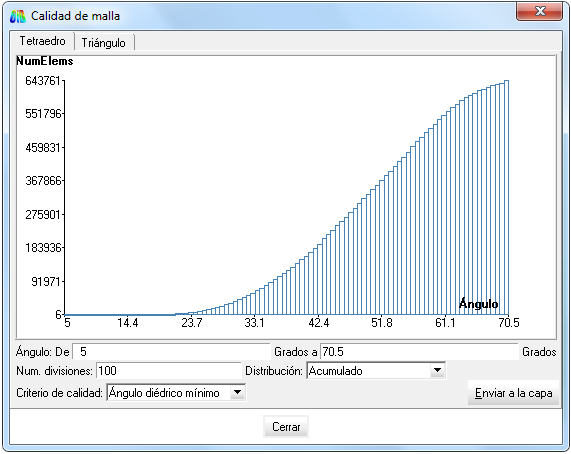
\includegraphics[scale=0.60]{img/cant_tetraedros}}
\caption{Calidad de la Malla - Tetraedros}
\label{calidadtetraedros}
\end{figure}

\begin{figure}[tbhp]
\centerline{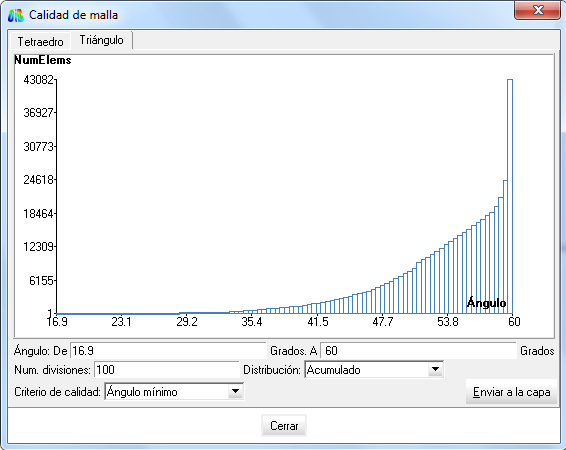
\includegraphics[scale=0.60]{img/cant_triangulos}}
\caption{Calida de la Malla - Triángulos}
\label{calidadtriangulos}
\end{figure}

\begin{figure}[tbhp]
\centerline{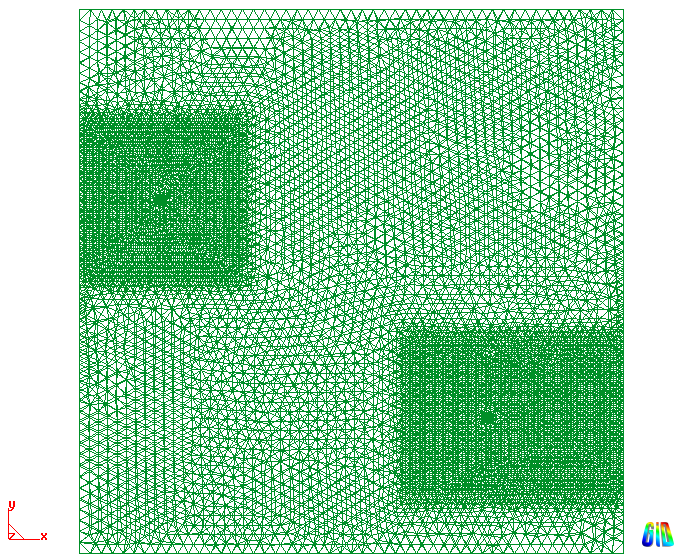
\includegraphics[scale=0.75]{img/contorno_malla_xy}}
\caption{Vista en el plano XY de la malla}
\label{contorno_malla_xy}
\end{figure}

%\begin{figure}[tbhp]
%\centerline{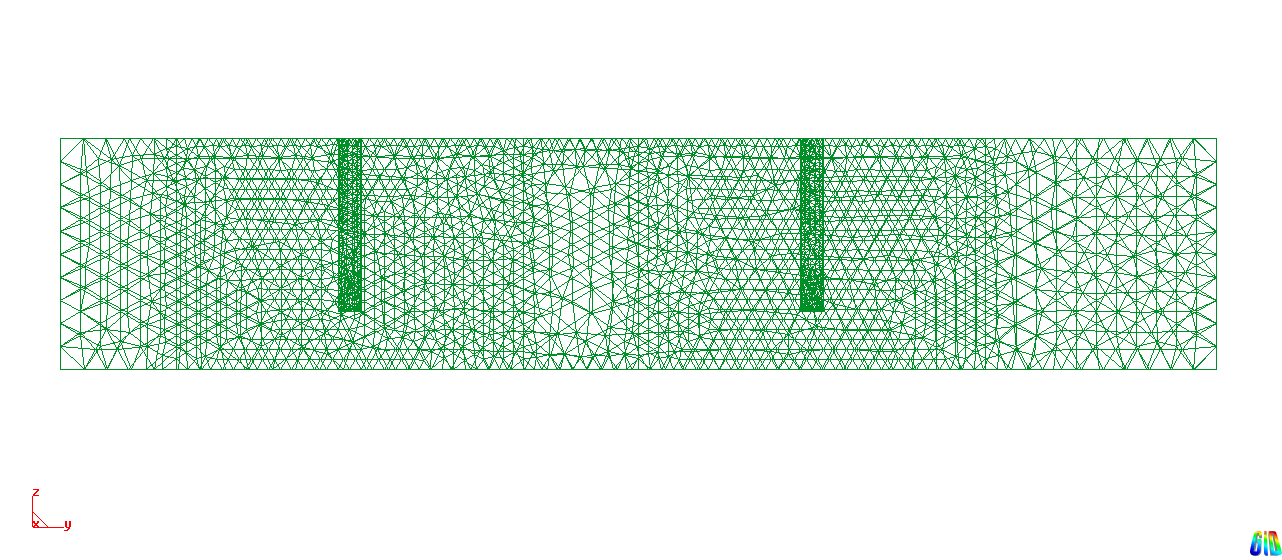
\includegraphics[scale=0.50]{img/contorno_malla_yz}}
%\caption{Vista en el plano YZ de la malla}
%\label{contorno_malla_yz}
%\end{figure}

\begin{figure}[tbhp]
\centerline{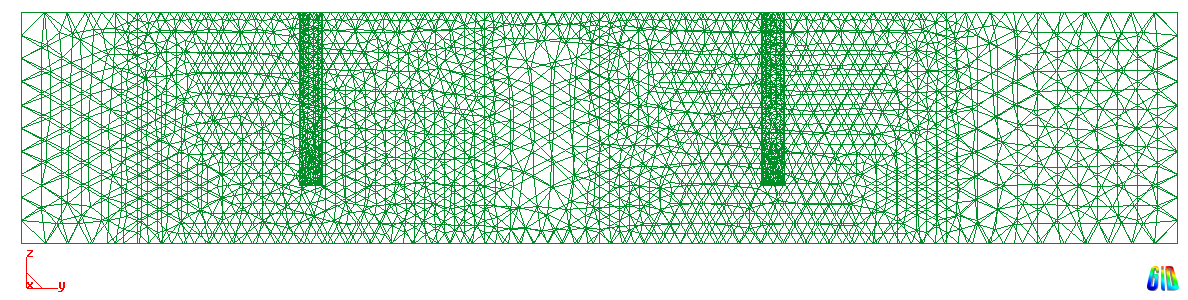
\includegraphics[scale=0.50]{img/contorno_malla_yz1}}
\caption{Vista en el plano YZ de la malla}
\label{contorno_malla_yz1}
\end{figure}

\begin{figure}[tbhp]
\centerline{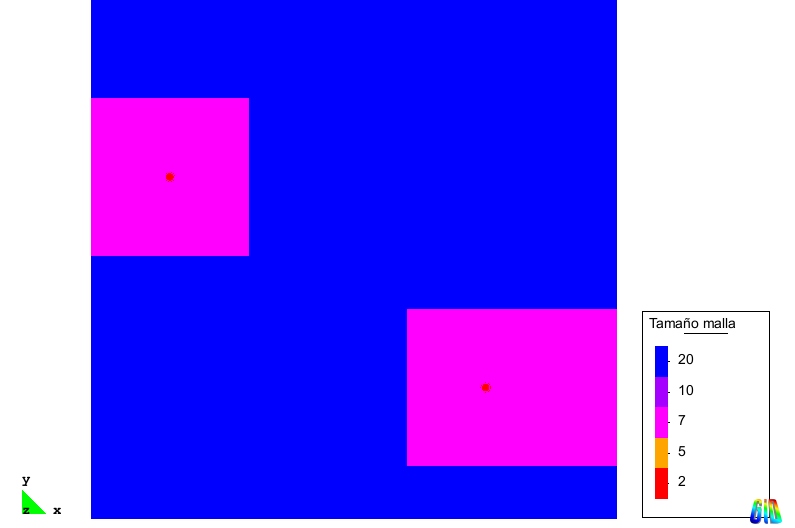
\includegraphics[scale=0.50]{img/tam_malla_xy}}
\caption{Tamaños de elementos de la malla - Vista en el plano XY}
\label{tam_malla_xy}
\end{figure}

\begin{figure}[tbhp]
\centerline{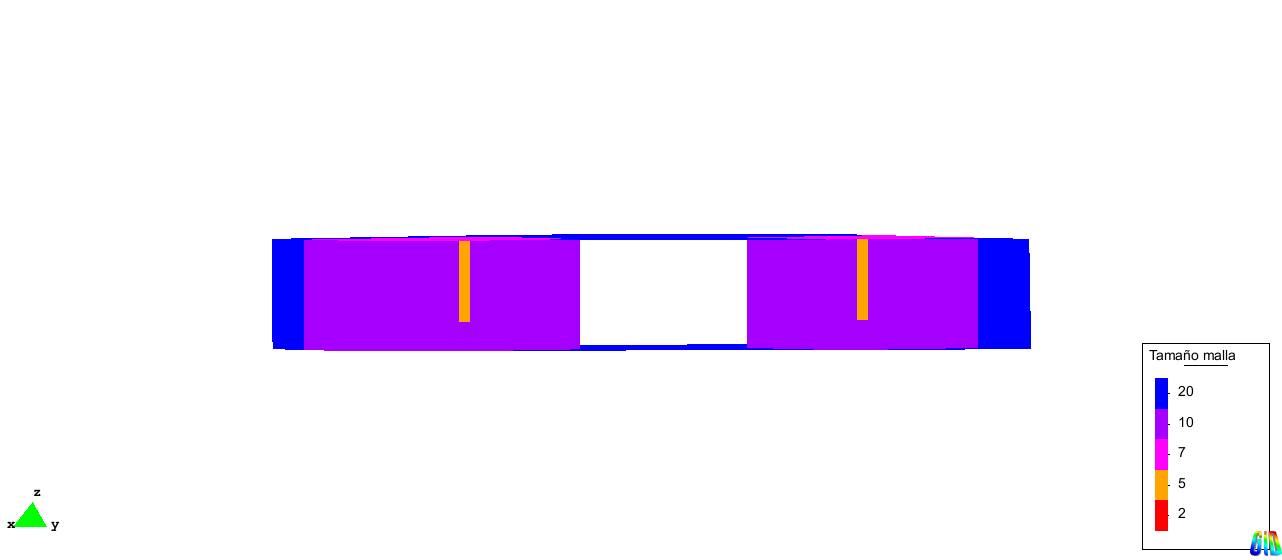
\includegraphics[scale=0.50]{img/tam_malla_pozo_interior}}
\caption{Tamaños de elementos de la malla - Corte transversal}
\label{tam_malla_pozo_interior}
\end{figure}
%
\subsection{Condiciones temporales}
describir como oelegimos en
%
%
\subsection{Ejecución}
cambiar el titulo esto es como se llevo a cabao la corrida

ver graficos en un nodo o punto la evolucion de una variable. -> point evolution ->velocity->module->elijo un nodo
%%%%%%%%%%%%%%%%%%%%%%%%%%%%%%%%%%%%%%%%%%%%%%%%%
%%%%%%%%%%%%%%%%%%%%%%%%%%%%%%%%%%%%%%%%%%%%%%%%%
%%%%%%%%%%%%%%%%%%%%%%%%%%%%%%%%%%%%%%%%%%%%%%%%%
\section{Resultados}
v(veloc) -> lineas de flujo/vect
p->equipotenciales
realizar cortes

lo que vamos a ver va a ser las equipotenciales (lineas de presion que son perpendiculares al flujo).siempre es contraria a la linea de velocidad
%%%%%%%%%%%%%%%%%%%%%%%%%%%%%%%%%%%%%%%%%%%%%%%%%
%%%%%%%%%%%%%%%%%%%%%%%%%%%%%%%%%%%%%%%%%%%%%%%%%
%%%%%%%%%%%%%%%%%%%%%%%%%%%%%%%%%%%%%%%%%%%%%%%%%
\section{Conclusiones}
si el mod respondio
que problemas tuvimos? ahi hacer mencion al pozo grande y tiempo de calculo...
pozo real vs pozo simulado
%%%%%%%%%%%%%%%%%%%%%%%%%%%%%%%%%%%%%%%%%%%%%%%%%
%%%%%%%%%%%%%%%%%%%%%%%%%%%%%%%%%%%%%%%%%%%%%%%%%
%%%%%%%%%%%%%%%%%%%%%%%%%%%%%%%%%%%%%%%%%%%%%%%%%
\end{document}